\documentclass[a4paper,10pt]{article}
\usepackage[utf8]{inputenc}
\usepackage{graphicx}
\usepackage{pdflscape}

% Title Page
\title{Software architecture \\ Assignment 2}
\author{ Dehouck Samuel, Delhaye Quentin \\}


\begin{document}
\maketitle

\section{Introduction}

In this project, we were asked to refactor (flawed) three-tier architecture that implements a web portal applicaton which allows to store and retreive informations about books, articles, etc. Moreover, we needed to identify the different flaws of
this architecture.\\
More precisely, we had to refactor the database layer in order to be able to easily insert a new format of database. The details of this new implementation will be detailed in the first section. Next, we will give the flaws that we found in the architecture.

\section{Refactoring}

For this project, we had to refactor the database layer in order to add a new database based on \textit{CSV} files. The original implementation didn't allow us to easily add this new layer and that is where the refactoring is done.
\newline
First, we needed to change some names to make them more precise: \textit{RawDatabase} became \textit{RawDataseSQL}, \textit{UserDatabase} \textit{UserDatabaseSQL}, \textit{RegularDatabase} \textit{RegularDatabaseSQL} and finally \textit{Database} \textit{DatabaseSQL}. 
\newline
In a second time, we added a new level of abstraction with some interfaces that are implemented by the SQL components inherit: \textit{RawDatabase}, \textit{UserDatabase}, \textit{RegularDatabase}.  We also created a new abstract 
class Database from which DatabaseSQL inherits. With this generic interfaces and the abstract class, it became much easier to add a new kind of database.
\newline
Finally, we created the \textit{CSV} database with some new classes \textit{RawDatabaseCSV}, \textit{UserDatabaseCSV} and \textit{RegularDatabase} that implement the corresponding interfaces and \textit{DatabaseCSV} inheriting from \textit{Database}.
\newline
All these classes have been reorganized in the new packages \textit{db.flatfile} and \textit{db.sql}.
\newline
The figure~\ref{fig:classesDiagram} present those modifications.

\begin{figure}[h]
 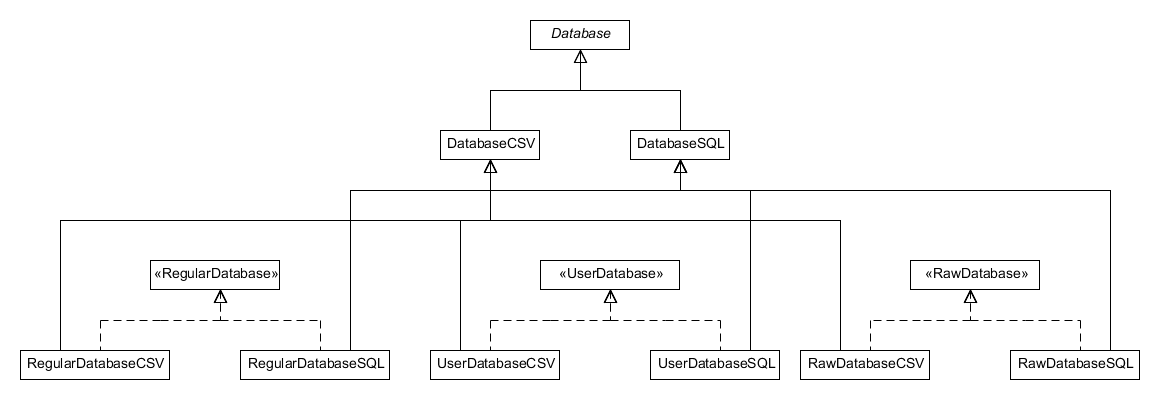
\includegraphics[width=\textwidth]{ClassDiagram.png}
 \caption{Classes diagram of the refactoring the database architecture.}
 \label{fig:classesDiagram}
\end{figure}

As we can see with this new architecture, it is much easier to add a new kind of database.
\newline

\pagebreak

Some others changes needed to be done in order to have a working implementation:
\begin{itemize}
	\item We apended a new line in the file \texttt{web\_portal.cfg} to specify the format of the database: \texttt{dbFormat=csv}, if a csv based database is to be used, \texttt{dbFormat=sql} in case SQL.
 \item The constructor of the class \textit{ApplicationFacade} has been modified to take the format into account.
 \item The constructor of the class \textit{DatabaseFacade} has been modified in the same way and now build the database accordingly.
 \item In order to store the user profiles into the database, a new method \textit{asCSV} has been added in the classes \textit{UserProfile} and children.
\end{itemize}

\section{Configuration}
Several files need to be changed to switch between the databases:
\begin{description}
\item[Inside \texttt{web\_portal.cfg}:] \texttt{dbUrl=/path/to/project/DB} and \texttt{dbFormat=csv}
\item[Inside \texttt{WebContent/WEB-INF/web.xml}:] \texttt{param-value=/path/to/project/web\_portal.cfg}
\end{description}


\section{Design flaws}

When we refactored the database layer, we found that the database needed to ask the \textit{UserProfile} to give its information in a format that it was possible to store (\textit{asSQL} and \textit{asCSV} methods). It clearly introduce some coupling that could be
avoided if the database could ask the \textit{UserProfile} to give a generic format of itself. Then, it would be the job of the database to convert it into \textit{SQL} or \textit{CSV} in order to store it.

An other problem is the coupling between the data objects and the database type.
All the constructors receive a resultset as a parameter, which is typical of usage of an SQL-type database.
Those constructors should be independant of the database type, i.e. receive a generic object as argument.
The translation from resultset to that structure should be done in the database layer.

Following the same idea, the \texttt{ui} package knows to much about the \texttt{data} package as well.
When the \texttt{AdministrationPage} wants to add information to the database, it first creates objects typed from the \texttt{data} package, and then sends them to the \texttt{ApplicationFacade} (which will forward them to the \texttt{DataBaseFacade}).
The user interface package should structure the data independently from the data package before sending it to the facade.


\section{Conclusion}
The application can now use \texttt{csv} database and adding new type of database is easier.
There is still a high degree of coupling between the layers that should be refactored.

%\tableofcontents
\end{document}          
